\documentclass[12pt]{article}

\usepackage{sbc-template}

% \usepackage[pdfpagelabels]{hyperref}
\usepackage{amsmath,amsthm,amsfonts,amssymb}
\usepackage{latexsym}
\usepackage[utf8]{inputenc}
\usepackage{textcase}
\usepackage{listings}
\usepackage[T1]{fontenc}

\usepackage{latexsym}

\usepackage{graphicx,url}

%\usepackage[brazil]{babel}
\usepackage[utf8]{inputenc}

\newcommand{\prog}[1]{
  \normalfont\ttfamily
  \begin{center}\begin{tabular}{l}
       #1
  \end{tabular} \end{center}
  \normalfont}

\newcommand{\proga}[1]{
 \normalfont\ttfamily
  \begin{tabbing}
        #1
   \end{tabbing}
 \normalfont}

\newcommand{\progfig}[1]{\parbox{.96\textwidth}{
  \normalfont\ttfamily
  {\small
  \parbox{\textwidth}{\begin{tabbing}
        #1
  \end{tabbing}}
}
  \normalfont}}

\newcommand{\progfigmed}[1]{\parbox{.65\textwidth}{
  \normalfont\ttfamily
  {\small
  \parbox{\textwidth}{\begin{tabbing}
        #1
  \end{tabbing}}
}
  \normalfont}}


\newcommand{\progfigsmall}[1]{\parbox{.44\textwidth}{
  \normalfont\ttfamily
  {\small
%  \begin{center}
  \parbox{.44\textwidth}{\begin{tabbing}
        #1
  \end{tabbing}}
%  \end{center}
}
  \normalfont}}

\newcommand{\progb}[1]{
  \normalfont\ttfamily
  {\small
  \begin{center}
  \parbox{\textwidth}{\begin{tabbing}
        #1
  \end{tabbing}}
  \end{center} }
  \normalfont}

\newcommand{\scripttag}[1]{\texttt{\scriptsize{(}}\textsl{\scriptsize{#1}}{\texttt{\scriptsize{)}}}}

\newcommand{\progn}[1]{
  \begin{center}
  \parbox{\textwidth}{\begin{tabbing}
        #1
  \end{tabbing}}
  \end{center} }



\newcommand{\progbb}[1]{
  \normalfont\ttfamily
  \begin{center}
  \shadowbox{\parbox{\textwidth}{\begin{tabbing}
        #1
  \end{tabbing}}}
  \end{center}
  \normalfont}

\newcommand{\progc}[1]{
  \normalfont\ttfamily
  \begin{center}
  \fbox{\parbox{\textwidth}{\begin{tabbing}
        #1
  \end{tabbing}}}
  \end{center}
  \normalfont}

\newcommand{\progcc}[1]{
  \normalfont\ttfamily
  \begin{center}
  \fbox{\begin{tabular}{p{4cm}}
        #1
  \end{tabular}}
  \end{center}
  \normalfont}

\newcommand{\progaa}[1]{
  \normalfont\ttfamily
  \begin{center}\begin{tabular}{ll}
       #1
  \end{tabular} \end{center}
  \normalfont}

\newcommand{\progaaa}[1]{
  \normalfont\ttfamily
  \begin{center}\begin{tabular}{lll}
       #1
  \end{tabular} \end{center}
  \normalfont}

\newcommand{\progeq}[1]{
  \normalfont\ttfamily
  \begin{center}\begin{tabular}{rcl}
       #1
  \end{tabular} \end{center}
  \normalfont}

\newcommand{\CT}{\text{\it CT\/}}
\newcommand{\CSSAT}{\text{\it CS-SAT\/}}
\newcommand{\ssat}{\text{\tt sat}}

\newcommand{\lcg}{\text{\it lcg\/}}

\newcommand{\Integer}{\text{\it Integer\/}}
\newcommand{\Bool}{\text{\it Bool\/}}
\newcommand{\Int}{\text{\it Int\/}}
\newcommand{\Char}{\text{\it Char\/}}
\newcommand{\Float}{\text{\it Float\/}}
\newcommand{\Double}{\text{\it Double\/}}

\newcommand{\True}{\text{\it True\/}}
\newcommand{\False}{\text{\it False\/}}

\newcommand{\Lit}{\text{\it Lit\/}}
\newcommand{\Inc}{\text{\it Inc\/}}
\newcommand{\IsZ}{\text{\it IsZ\/}}
\newcommand{\If}{\text{\it If\/}}
\newcommand{\Pair}{\text{\it Pair\/}}
\newcommand{\Term}{\text{\it Term\/}}

\newcommand{\eval}{\text{\it eval\/}}
\newcommand{\iinsert}{\text{\it insert\/}}

\newcommand{\MMo}{{\tt MMo}}

\newcommand{\genn}[1]{\bar{\bar{#1}}}
\newcommand{\abrgenn}[1]{\|#1\|}

\newcommand{\T}{\text{\it T\/}}
\newcommand{\Tu}{\text{\it T1\/}}
\newcommand{\Td}{\text{\it T2\/}}
\newcommand{\test}{\text{\it test\/}}
\newcommand{\sat}{\text{\it sat\/}}
\newcommand{\sats}{\text{\it sats\/}}

\newcommand{\Eq}{\text{\it Eq\/}}

\newcommand{\TEq}{\rightarrowtail}
\newcommand{\TEqD}{\rotatebox[origin=c]{270}{\Large \rightarrowtail}}
\newcommand{\tti}{\texttt{i}}
\newcommand{\ttk}{\texttt{k}}
\newcommand{\ttx}{\texttt{x}}
\newcommand{\tty}{\texttt{y}}
\newcommand{\ttp}{\texttt{p}}
\newcommand{\tts}{\texttt{s}}
\newcommand{\ttr}{\texttt{r}}
\newcommand{\tta}{\texttt{a}}
\newcommand{\ttc}{\texttt{c}}
\newcommand{\ttconst}{\texttt{const}}
\newcommand{\ttinfo}{\texttt{info}}

% \newcommand{\INST}{\text{\tt INST}}
% \newcommand{\ABS}{\text{\tt ABS}}
% \newcommand{\GEN}{\text{\tt GEN}}
% \newcommand{\VAR}{\text{\tt VAR}}
% \newcommand{\PVAR}{\text{\tt PVAR}}
% \newcommand{\SKO}{\text{\tt VAR-SKO}}
% \newcommand{\UNI}{\text{\tt VAR-UNI}}
% \newcommand{\FUN}{\text{\tt FUN}}
% \newcommand{\CONS}{\text{\tt CONS}}
% \newcommand{\LAM}{\text{\tt LAM}}
% \newcommand{\APP}{\text{\tt APP}}
% \newcommand{\LET}{\text{\tt LET}}
% \newcommand{\LETA}{\text{\tt LETA}}
% \newcommand{\CASE}{\text{\tt CASE}}
% \newcommand{\BIND}{\text{\tt BIND}}
% \newcommand{\EEMPTY}{\text{\tt EMPTY}}
% \newcommand{\IMPROVE}{\text{\tt IMPROVE}}
% \newcommand{\PATVAR}{\text{\tt PAT-VAR}}
% \newcommand{\PAT}{\text{\tt PAT}}
% \newcommand{\TPAT}{\text{\tt TPAT}}
% \newcommand{\INFER}{\text{\tt INFER}}
% \newcommand{\PATCONS}{\text{\tt PAT-CONS}}
% \newcommand{\ALTS}{\text{\tt ALTS}}
% \newcommand{\ALT}{\text{\tt ALT}}
% \newcommand{\MAIN}{\text{\tt MAIN}}
% \newcommand{\alts}{\text{\tt alts}}
% \newcommand{\alt}{\text{\tt alt}}
% \newcommand{\pat}{\text{\tt pat}}

%%%%%%%%%%%%%%%%%%%%%%%%%%%%%%%%%%%%%%%%%%%%%%%%%%%%%%%%%%%%%%%%%%%%%%%%%%%%%
%                                                                           %
% DEFINITIONS OF SYMBOL-PRODUCING COMMANDS                                  %
%                                                                           %
%    TLA+      LaTeX                                                        %
%    symbol    command                                                      %
%    ------    -------                                                      %
%    =>        \implies                                                     %
%    <:        \ltcolon                                                     %
%    :>        \colongt                                                     %
%    ==        \defeq                                                       %
%    ..        \dotdot                                                      %
%    ::        \coloncolon                                                  %
%    =|        \eqdash                                                      %
%    ++        \pp                                                          %
%    --        \mm                                                          %
%    **        \stst                                                        %
%    //        \slsl                                                        %
%    ^         \ct                                                          %
%    \A        \A                                                           %
%    \E        \E                                                           %
%    \AA       \AA                                                          %
%    \EE       \EE                                                          %
%%%%%%%%%%%%%%%%%%%%%%%%%%%%%%%%%%%%%%%%%%%%%%%%%%%%%%%%%%%%%%%%%%%%%%%%%%%%%
% \newcommand{\implies}{\Rightarrow}
\newcommand{\ltcolon}{\mathrel{<\!\!\mbox{:}}}
\newcommand{\colongt}{\mathrel{\!\mbox{:}\!\!>}}
\newcommand{\defeq}{\;\mathrel{\smash   %% keep this symbol from being too tall
    {{\stackrel{\scriptscriptstyle\Delta}{=}}}}\;}
\newcommand{\dotdot}{\mathrel{\ldotp\ldotp}}
\newcommand{\coloncolon}{\mathrel{::\;}}
\newcommand{\eqdash}{\mathrel = \joinrel \hspace{-.28em}|}
\newcommand{\pp}{\mathbin{++}}
\newcommand{\mm}{\mathbin{--}}
\newcommand{\stst}{*\!*}
\newcommand{\slsl}{/\!/}
\newcommand{\ct}{\hat{\hspace{.4em}}}
\newcommand{\A}{\forall}
\newcommand{\E}{\exists}
\renewcommand{\AA}{\makebox{$\raisebox{.05em}{\makebox[0pt][l]{%
   $\forall\hspace{-.517em}\forall\hspace{-.517em}\forall$}}%
   \forall\hspace{-.517em}\forall \hspace{-.517em}\forall\,$}}
\newcommand{\EE}{\makebox{$\raisebox{.05em}{\makebox[0pt][l]{%
   $\exists\hspace{-.517em}\exists\hspace{-.517em}\exists$}}%
   \exists\hspace{-.517em}\exists\hspace{-.517em}\exists\,$}}
\newcommand{\whileop}{\.{\stackrel
  {\mbox{\raisebox{-.3em}[0pt][0pt]{$\scriptscriptstyle+\;\,$}}}%
  {-\hspace{-.16em}\triangleright}}}

% Commands are defined to produce the upper-case keywords.
% Note that some have space after them.
\newcommand{\TLA}{TLA\textsuperscript{+} }
\newcommand{\TLAA}{TLA\textsuperscript{+}}
\newcommand{\FANCYA}{\textbf{$\mathcal{A}$} }
\newcommand{\FANCYAA}{\textbf{$\mathcal{A}$}}
\newcommand{\trabalhando}{"trabalhando"}
\newcommand{\preparado}{"preparado"}
\newcommand{\cometido}{"cometido"}
\newcommand{\abortado}{"abortado"}

\newcommand{\ASSUME}{\textsc{assume }}
\newcommand{\ASSUMPTION}{\textsc{assumption }}
\newcommand{\AXIOM}{\textsc{axiom }}
\newcommand{\BOOLEAN}{\textsc{boolean }}
\newcommand{\CASE}{\textsc{case }}
\newcommand{\CONSTANT}{\textsc{constant }}
\newcommand{\CONSTANTS}{\textsc{constants }}
\newcommand{\ELSE}{\settowidth{\symlength}{\THEN}%
   \makebox[\symlength][l]{\textsc{ else}}}
\newcommand{\EXCEPT}{\textsc{ except }}
\newcommand{\EXTENDS}{\textsc{extends }}
\newcommand{\FALSE}{\textsc{false}}
\newcommand{\IF}{\textsc{if }}
\newcommand{\IN}{\settowidth{\symlength}{\LET}%
   \makebox[\symlength][l]{\textsc{in}}}
\newcommand{\INSTANCE}{\textsc{instance }}
\newcommand{\LET}{\textsc{let }}
\newcommand{\LOCAL}{\textsc{local }}
\newcommand{\MODULE}{\textsc{module }}
\newcommand{\OTHER}{\textsc{other }}
\newcommand{\STRING}{\textsc{string}}
\newcommand{\THEN}{\textsc{ then }}
\newcommand{\THEOREM}{\textsc{theorem }}
\newcommand{\LEMMA}{\textsc{lemma }}
\newcommand{\PROPOSITION}{\textsc{proposition }}
\newcommand{\COROLLARY}{\textsc{corollary }}
\newcommand{\TRUE}{\textsc{true}}
\newcommand{\VARIABLE}{\textsc{variable}}
\newcommand{\VARIABLES}{\textsc{variables}}
\newcommand{\WITH}{\textsc{ with }}
\newcommand{\WF}{\textrm{WF}}
\newcommand{\SF}{\textrm{SF}}
\newcommand{\CHOOSE}{\textsc{choose }}
\newcommand{\ENABLED}{\textsc{enabled }}
\newcommand{\UNCHANGED}{\textsc{unchanged }}
\newcommand{\SUBSET}{\textsc{subset }}
\newcommand{\UNION}{\textsc{union }}
\newcommand{\DOMAIN}{\textsc{domain }}
% Added for tla2tex
\newcommand{\BY}{\textsc{by }}
\newcommand{\OBVIOUS}{\textsc{obvious }}
\newcommand{\HAVE}{\textsc{have }}
\newcommand{\QED}{\textsc{qed }}
\newcommand{\TAKE}{\textsc{take }}
\newcommand{\DEF}{\textsc{ def }}
\newcommand{\HIDE}{\textsc{hide }}
\newcommand{\RECURSIVE}{\textsc{recursive }}
\newcommand{\USE}{\textsc{use }}
\newcommand{\DEFINE}{\textsc{define }}
\newcommand{\PROOF}{\textsc{proof }}
\newcommand{\WITNESS}{\textsc{witness }}
\newcommand{\PICK}{\textsc{pick }}
\newcommand{\DEFS}{\textsc{defs }}
\newcommand{\PROVE}{\settowidth{\symlength}{\ASSUME}%
   \makebox[\symlength][l]{\textsc{prove}}\@s{-4.1}}%
  %% The \@s{-4.1) is a kludge added on 24 Oct 2009 [happy birthday, Ellen]
  %% so the correct alignment occurs if the user types
  %%   ASSUME X
  %%   PROVE  Y
  %% because it cancels the extra 4.1 pts added because of the
  %% extra space after the PROVE.  This seems to works OK.
  %% However, the 4.1 equals Parameters.LaTeXLeftSpace(1) and
  %% should be changed if that method ever changes.
\newcommand{\SUFFICES}{\textsc{suffices }}
\newcommand{\NEW}{\textsc{new }}
\newcommand{\LAMBDA}{\textsc{lambda }}
\newcommand{\STATE}{\textsc{state }}
\newcommand{\ACTION}{\textsc{action }}
\newcommand{\TEMPORAL}{\textsc{temporal }}
\newcommand{\ONLY}{\textsc{only }}              %% added by LL on 2 Oct 2009
\newcommand{\OMITTED}{\textsc{omitted }}        %% added by LL on 31 Oct 2009
% \newcommand{\@pfstepnum}[2]{\ensuremath{\langle#1\rangle}\textrm{#2}}
\newcommand{\bang}{\@s{1}\mbox{\small !}\@s{1}}


\sloppy

\title{Epecificação formal e prototipação de controlador de sitema de
  bombeamento de água}

\author{Gabriela Moreira Mafra\inst{1}}

\address{Departamento de Ciência da Computação \\Centro de Ciências Tecnológicas \\Universidade do Estado de Santa Catarina (UDESC)\\Joinville, SC -- Brasil
  \email{\{gabrielamoreiramafra@gmail.com\}}
}

\begin{document}

\maketitle

\begin{resumo}
 Estações de bombeamento de água consomem energia em alto volume, abrindo espaço
 para otimização desse custo energético de acordo com as variações do uso da
 água. O controle das bombas com esse objetivo é feito sob diversas restrições,
 que precisam ser validadas por diferentes entidades. Propõe-se uma
 especificação de sistema de controle para tais estações em uma liguagem de
 especificação formal, fornecendo vantagens de verificação de restrições. Um
 protótipo executável gerado a partir da especificação e adiciona-se, por
 fim, um módulo de comunicação MQTT a fim de tornar o protótipo viável em uma
 rede de sensores de baixo consumo. 
\end{resumo}

\begin{abstract}
 Water pump stations have a high energy consumption volumes, opening room for
 enery cost optimization according to variations on water usage. Pumo control
 with this objective is done under many restrictions, which need to be validated
 by different enitities. A control system specification for this stations is
 proposed using a formal specification language, providing advantages on
 restriction validations. An executable prototype is generated from the
 specification, and lastly, a comunnication module using the MQTT protocol is
 added, making it viable for the prototype to be used whithin a low power
 sensor network.
\end{abstract}

\begin{keyword}
  Internet of Things, Formal Methods, Pump Control, Temporal Logic of Actions, MQ Telemetry Transport
\end{keyword}
  
\section{Introdução}

Conforme \cite{feng}, o gasto com energia elétrica em estações de bombeamento
representam o maior gasto de energia elétrica de algumas indústrias como no
setor metalúrgico. O controle das bombas de água precisa manter os níveis de
água dentro de uma margem estabelecida, ao passo que esse mesmo nível varia
conforme o uso. O custo energético se dá pelo ato de desligar e ligar as
bombas, assim como mantê-las ligadas. Visando minimizar tal custo, os mecanismos
de controle avaliam as mudanças no nível de água e determinam quais bombas ligar
ou desligar.

Os sistemas de bombeamento podem ser significantemente heterogêneos, como é o
caso da estação estudada em \cite{pumps}. Nessa estação, bombas diferentes tem
custos associados diferentes, e há uma necessidade de equiílibrio de uso entre
bombas semelhantes. Os autores propõem um sistema de controle considerando essas
restrições, porém não apresentam nenhuma evidência ou prova de que foram
atendidas além da própria interpretação do código. O atendimento a essas
restrições precisou ser avaliado por governos locais, tamanha é sua importância.

Nesse cenário, propõe-se uma forma alternativa de definição desse sistema de
bombeamento, dada pela representação em uma linguagem de especificação formal.
Nessa estrutura, é possível validar diversas propriedades, tais quais as
restrições impostas, verificando que estas são atendidas em todos os estados
possíveis dentro do especificado.

Utilizando a linguagem de especificação \TLA - que tem sido difundida e possui
casos de aplicação relevantes como na Amazon \cite{amazon} - é possível
explicitar as restrições na própria especificação, usando uma sintaxe matemática
familiar. A principal vantagem da utilização dessa linguagem para a
representação é tornar mais fácil e confiável a validação do atendimento às
restrições.

Uma especificação formal, por si só, não permite uma execução em um sistema real
ou simulado para uma validação empírica ou para a própria aplicação real. Mas
utilizando um tradutor como o proposto em \cite{tcc}, se faz possível a obtenção
de um protótipo na linguagem de programação Elixir, que por sua vez pode ser
executado e aplicado.

Assim, propõe-se a especificação formal para o sistema de controle apresentado
em \cite{pumps}, a geração de código a partir dessaa especificação e a adaptação
desse protótipo para um sistema real, onde os elementos se comunicam com o
protocolo MQTT.

\subsection{Objetivo}

O objetivo deste trabalho se dá pela geração de um protótipo de sistema de
controle de bombeamento de água equivalente ao proposto em \cite{pumps} a partir
de uma especificação formal do algoritmo de controle.

\subsubsection{Objetivos Específicos}
\begin{itemize}
  \item Especificar o algoritmo de controle proposto em \cite{pumps} usando a liguagem \TLA;
  \item Gerar código executável em Elixir a partir dessa especificação, usando a
    ferramenta proposta em \cite{tcc};
  \item Adicionar módulo de comunicação com protocolo MQTT para receber dados de
    sensores;
  \item Simular o envio de dados de sensores, verificando se as reações do
    controlador estão de acordo com o esperado para o algoritmo.
\end{itemize}

\section{Trabalhos Relacionados}

O principal trabalho relacionado a este é a própria proposta do algoritmo aqui
especificado \cite{pumps}. No trabalho, os diversos fatores de uma estação de
bombeamento especifica, localizada na China, são considerados em uma otimização
do processo de controle das bombas de água. Para obter o algoritmo, é feita uma
simulação do ambiente, onde o fluxo de água é simulado a partir da capacidade
das bombas, e um algoritmo genético faz a seleção do controlador ótimo. Os
principais elementos do algoritmo resultante é dado na notação ANSI C.

Outros trabalhos envolvendo Internet das coisas e controle de estações de
bombeamento já foram feitos, indicando a relevância desse tipo de aplicação.
\cite{feng} propõe um sistema de monitoramento de saúde e sustentabiliade de
vários elementos da estação, envolvendo centenas de sensores. O estudo em
\cite{hotwater} propõe um sistema de controle para bombeamento de água quente,
onde existem novas otimizações a serem feitas, como a mantenabilidade da
temperatura da água.

Em termos de especificar formalmente esse tipo de sistema, um trabalho que
tangibiliza a ideia é feito em \cite{gas}. Os autores propõe o uso de uma
combinação entre métodos de especificação formais (utilizando Z e B) e
semi-formais como UML ou SDL. Eles então aplicam essa ideia em um estudo de caso
para uma estação de gás, que possui elementos comuns com estações de bombeamento
de água, como as próprias bombas.

\section{Abordagem Proposta}

Dados os objetivos específicos, apresenta-se aqui o processo de elaboração e uma
descrição detalhada de cada um dos artefatos produzidos.

\subsection{Especificação Formal}

O primeiro passo para a nova representação e prototipação do algoritmo de
controle base (dado em \cite{pumps}) é a própria especificação formal em \TLA
desse algoritmo. A tradução é feita de forma manual e é complexa, já que se
tratam de estruturas de representação bastante diferentes. A representação usada
na proposta original, ANSI C, é procedural; enquanto a representação em \TLA é
declarativa. Cada ação, dada por uma sequência de passos, é transformada em na
definição de transições de estado válidas.

Algumas restrições tratadas na representação original de forma implícita são
deixadas explícitas na especificação em \TLA. Um exemplo é a prioridade das
bombas, que é originalmente definida pela ordem de iteração $i=0..n$ e, em \TLA,
é dada como uma das condições para a transição ser válida. A especificação dessa
priorização em ANSI C se econtra na Figura \ref{fig:activate_ansi}, e a versão
em \TLA se encontra na Figura \ref{fig:activate_tla}.

\begin{figure}[h]
\begin{center}
  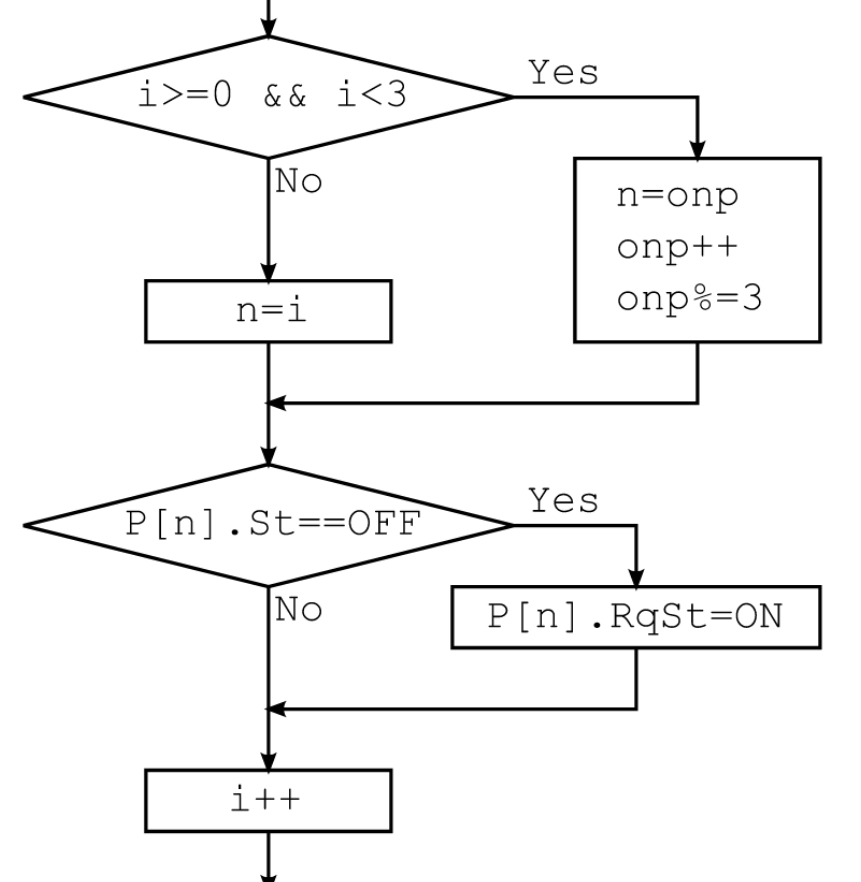
\includegraphics[width=0.4\textwidth]{activate_ansi.png}
\end{center}
  \caption{Especificação da priorização de bombas a serem ativadas em ANSI C.
    Fonte: \cite{pumps}}
  \label{fig:activate_ansi}
\end{figure}

\begin{figure}[h]
\begin{center}
  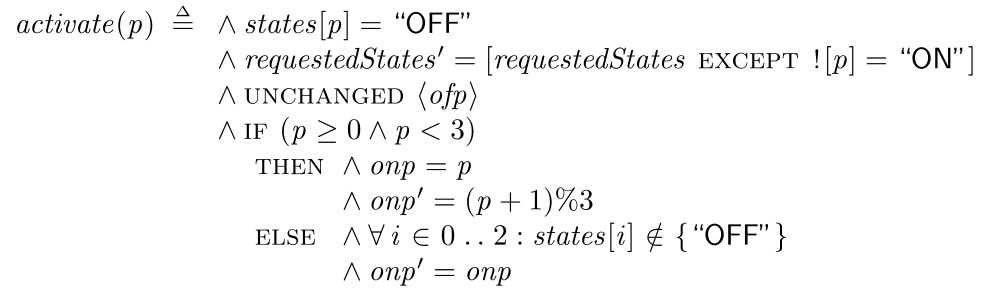
\includegraphics[width=0.9\textwidth]{activate_tla.png}
\end{center}
  \caption{Especificação da priorização de bombas a serem ativadas em \TLA.
    Fonte: autora}
  \label{fig:activate_tla}
\end{figure}

Na especificação em \TLA, se explicita que as bombas de número 4 acima só podem
ser ativadas se as bombas com menor custo associado (de 1 a 3) estiverem
desligadas. Isto é garantido pela condição $\A i \in 0..2 : states[i] \notin \{"OFF"\}$.

Uma vez que a especificação foi finalizada, algumas verificações simples foram
rodadas com o model checker TLC, verificando que o comportamento era conforme o
esperado e fazendo os ajustes necessários. Destaca-se que esse processo de
tradução manual é onde se concentra a maior parte do trabalho, enquanto o
restante é obtido a partir dessa especificação.

\subsection{Geração de Código}

Com a especificação finalizada, é possível gerar código na linguagem de
programação Elixir com a ferramenta proposta em \cite{tcc}. O trabalho justifica
a escolha da liguagem Elixir para a tradução com pontos relevantes, como a
proximidade com a especificação, que torna o código mais fácil de entender e
correlacionar com o artefato original; e a portabilidade dada pela máquina
virtual de Erlang BEAM (usada por Elixir). Este segundo ponto é de extrema valia para
o trabalho aqui proposto, já que possibilita que o protótipo gerado seja
executado em dispositivos condizentes com o contexto, como um Raspberry Pi.

Para gerar o código, vários ajustes foram necessários na ferramenta de tradução.
A ferramenta é apenas um protótipo inicial, e não suporta toda a gramática da
linguagem \TLA. Assim, novas regras de tradução precisaram ser criadas,
contribuindo para a maturidade da ferramenta. Com todos os ajustes feitos, o
protótipo pode ser gerado com sucesso, sem necessidade de alterações manuais
no arquivo gerado.

\subsection{Comunicação}

O código gerado prevê a implementação de uma forma de comunicação com entradas
externas, provido pela própria ferramenta de tradução. Essa comunicação é feita
por um processo denominado oráculo, que é responsável por receber entradas
sempre que o sistema em si não conseguir determinar o que fazer - isto é, quando
se necessita uma entrada externa. No caso da estação de bombeamento, as entradas
externas são:

\begin{itemize}
\item Aumento ou diminuição do nível de água do reservatório;
\item Estado de cada uma das bombas de água (saudável ou danificado).
\end{itemize}

O oráculo é um processo a parte, que se comunica com o sistema através de canais
do Elixir, que podem se comunicar com através da rede. Esse tipo de comunicação
não seria adequado para receber informações de sensores simples, que podem não
ser capazes de executar uma máquina virual BEAM. Considerando isso, é adicionado
um novo módulo de comunicação que recebe as leituras dos sensores utilizando o
protocolo MQTT. Esse módulo pode ser executado no próprio hardware do
controlador, dentro de uma BEAM, sendo assim capaz de se comunicar com o oráculo
pelos canais de Elixir.

A utilização do protocolo MQTT se justifica pela combinação de sua
compatibilidade em sistemas de Internet das coisas e sua interface simples do
tipo Publicador-Subscritor. O pacote Tortoise \cite{tortoise} oferece um cliente
MQTT para Elixir, usado para inscrever o módulo de comunicação nos tópicos
usados pelos sensores. Como broker, utilizou-se o Mosquitto \cite{mosquitto},
executado também no controlador.

Os sensores são simulados, uma vez que a obtenção de dados reais ou
experimentação no ambiente não são viáveis. Assim, a publicação das mensagens de
leitura dos sensores é enviada pelo próprio cliente do Mosquitto, com o
executável $\texttt{mosquitto\_pub}$.

Usando o padrão do protocolo MQTT, os tópicos foram criados como:
\begin{itemize}
  \item $\texttt{water\_level}$ recebendo mensagens ``up'' ou ``down''
  \item $\texttt{pumps/+/state}$ recebendo mensagens ``healthy'' ou ``damaged''
\end{itemize}

A leitura do nível de água é abstraída para facilitar a simulação. No ambiente
real, haveriam leituras dos 11 sensores dispostos no reservatório, informando se
a leitura é ``com água'' ou ``sem água''. A modificação para esse modelo seria
trivial, e a motivação para a simplificação em uma única leitura de ``up'' ou
``down'' garante que as alterações simuladas sejam condizentes com a realidade.
Assim, quando uma leitura ``up'' é feita, considera-se que o nível da água
aumentou a distância entre os dois sensores na região de alteração, uma vez que
essas seriam as mudanças de fato detectadas no sistem real.

\section{Resultados}

O sistema final inclui 3 processos Elixir e um broker MQTT a serem rodados no
controlador, e a publicação de leituras de sensores por um cliente MQTT
qualquer. Os testes foram simulados em um ambiente com rede Ethernet, devido a
limitações de hardware disponíveis, mas podem ser utilizados com qualquer
interface de rede. A comunicação entre o controlador e os sensores foi feita com
TCP/IP, usado pelo protocolo MQTT. As ações são impressas na tela do próprio
controlador para a simplificação do escopo, e é trivial usar o mesmo cliente,
Tortoise, para comunicar as ações com o protocolo MQTT em um novo tópico aos
atuadores que estariam disponíveis no ambiente real.

O controlador pode ser executado em qualquer sistema com suporte à máquina BEAM
e a um broker MQTT. Um dispositivo recomendado é o Raspberry Pi, com seu sistema
operacional próprio que atende essas restrições. Destaca-se que o tipo de
hardware e local onde o controlador está sendo executado é transparente, uma vez
que toda comunicação entre controlador e sensores é feita através do protocolo
MQTT.

A especificação formal em \TLA e todo o código para o controlador, incluindo o
módulo de comunicação, se encontra disponível em \url{https://github.com/GabrielaMafra/pump-station}.

\section{Considerações Finais}

A conversão de representação do algoritmo de controle para uma linguagem de
especificação se mostrou benéfica por explicitar restrições do sistema e
perimitir validações de diversas propriedades. Adicionalmente, a geração de
código a partir dessa especificação economiza o trabalho manual que seria
necessário para implementar uma versão executável do algoritmo de controle -
necessária quando este é especificado em outras representações não formais.

O protótipo gerado, em conjunto com o módulo de comunicação MQTT, se mostraram
funcionais nos testes realizados. Os testes, contudo, foram realizados com dados
arbitrários, já que os dados reais de leituras de sensores na estação
considerada não estão disponíveis.

Considera-se este trabalho como uma exemplificação de uma forma mais robusta de
propor soluções, aplicando ao contexto de Internet das coisas. Os benefícios
proporcionados por especificar formalmente os algoritmos são ainda mais notáveis
em sistemas complexos e distribuídos, sendo este caso de aplicação uma
demonstração do procedimento e das resultantes de usar especificação formal em
conjunto da geração de código.

\subsection{Trabalhos Futuros}

Na vertente de aproveitar por completo a especificação formal do algoritmo de
controle, seria interessante listar uma série de propriedades desejadas nesse
tipo de sistema e verificá-las para o algoritmo proposto. Neste trabalho, só
foram especificadas propriedades específicas aos estados de execução, inseridas
na própria especificação. Verificações mais complexas podem ser feitas com o uso
de fórmulas de lógica temporal.

Em termos de exploração e fomentação da prática de especificar software
formalmente, seria relevante ver trabalhos análogos a este em diferentes áreas
de aplicação, principalmente em sistemas distribuídos, onde o valor gerado pelas
verificações é ainda maior.

\bibliographystyle{abnt-alf}
\nocite{*}
\bibliography{main}

\end{document}
